\iffalse
\documentclass[a4paper,10pt]{report}
\usepackage[latin1]{inputenc}
\usepackage{amsmath}
\usepackage{amsmath,bm}
\usepackage{amsthm}
\usepackage{mathtools}
\usepackage{amsfonts}
\usepackage{amssymb}
\usepackage{graphicx}
\usepackage{array}
\usepackage{booktabs}
\usepackage{hyperref}
\usepackage{multicol}
\usepackage[margin=0.5in]{geometry}
\usepackage{karnaugh-map}
\usepackage[framemethod=tikz]{mdframed}
\newcommand{\myvec}[1]{\ensuremath{\begin{pmatrix}#1\end{pmatrix}}}
\let\vec\mathbf
\newcommand{\mydet}[1]{\ensuremath{\begin{vmatrix}#1\end{vmatrix}}}
\providecommand{\mbf}{\mathbf}
\providecommand{\pr}[1]{\ensuremath{\Pr\left(#1\right)}}
\providecommand{\qfunc}[1]{\ensuremath{Q\left(#1\right)}}
\providecommand{\sbrak}[1]{\ensuremath{{}\left[#1\right]}}
\providecommand{\lsbrak}[1]{\ensuremath{{}\left[#1\right.}}
\providecommand{\rsbrak}[1]{\ensuremath{{}\left.#1\right]}}
\providecommand{\brak}[1]{\ensuremath{\left(#1\right)}}
\providecommand{\lbrak}[1]{\ensuremath{\left(#1\right.}}
\providecommand{\rbrak}[1]{\ensuremath{\left.#1\right)}}
\providecommand{\cbrak}[1]{\ensuremath{\left\{#1\right\}}}
\providecommand{\lcbrak}[1]{\ensuremath{\left\{#1\right.}}
\providecommand{\rcbrak}[1]{\ensuremath{\left.#1\right\}}}
\begin{document}
\raggedright{
\includegraphics[scale=0.07]{logo.jpg}}\hspace{12.425cm}\raggedleft FWC22025\vspace{2mm}\\
\centering\Large\textbf{MATRICES-CIRCLES}\vspace{5mm}
\begin{multicols}{2}
\centering \large\textsc{C}\footnotesize\textsc{ONTENTS}\vspace{5mm}\\
\raggedright\large\textbf{1\hspace{1cm}Problem}\hspace{5.2cm}1\vspace{5mm}\\
\raggedright\large\textbf{2\hspace{1cm}Solution}\hspace{5.25cm}1\vspace{5mm}\\
\raggedright\large\textbf{3\hspace{1cm}Construction}\hspace{4.25cm}2\vspace{5mm}\\
\centering \large\textsc{1  P}\footnotesize\textsc{ROBLEM}\vspace{5mm}\\
\raggedright\large{
\fi
	Construct a tangent to a circle of radius 4cm from a point on the concentric circle of radius 6cm and measure its length. Also verify the measurement by actual calculation.
	\\
	\solution See Fig. 
		\ref{fig:10/11/2/2}.
	\begin{figure}[!ht]
		\centering
 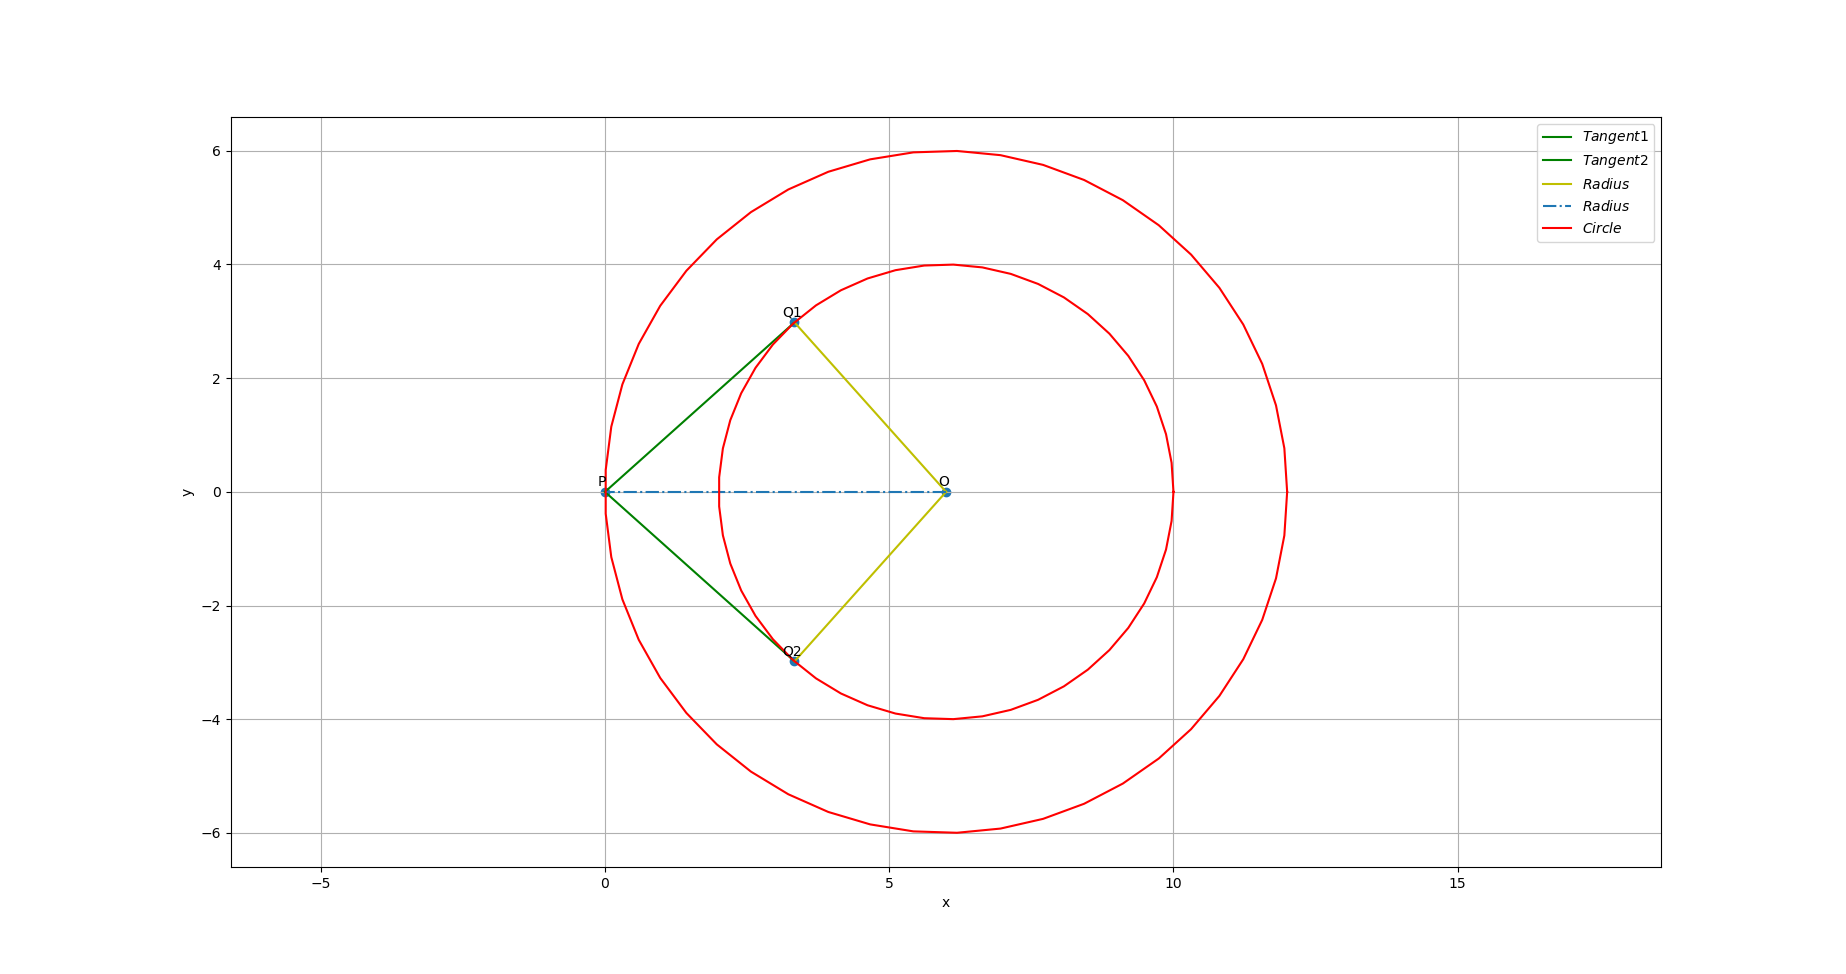
\includegraphics[width=\columnwidth]{chapters/10/11/2/2/figs/main.png}
		\caption{}
		\label{fig:10/11/2/2}
  	\end{figure}
\iffalse
	}\vspace{5mm}\\
\centering \large\textsc{2  S}\footnotesize\textsc{OLUTION}\vspace{5mm}\\
\raggedright\large{Consider a point P on the circle of radius 6 cm is at the origin and the center of circle is at d distance from P (where d=6).}\vspace{2mm}\\
\raggedright\large{Two tangents can be drawn from point P on to the circle of radius 4 cm which is concentric to the circle of radius 6 cm and let the point of contacts be Q1 and Q2.}\vspace{2mm}\\
\raggedright\large{The point of intersection of line \begin{align}L: \quad \vec{x} = \vec{q} + \mu \vec{m} \quad \mu \in \mathbb{R}\end{align} with the conic section \begin{align}\vec{x}^{\top}\vec{V}\vec{x}+2\vec{u}^{\top}\vec{x}+f=0\end{align} is given by \begin{align}\vec{x}_i = \vec{q} + \mu_i \vec{m}\end{align}}
where
\begin{multline}
\mu_i = \frac{1}
{
\vec{m}^{\top}\vec{V}\vec{m}
}
\lbrak{-\vec{m}^{\top}\brak{\vec{V}\vec{q}+\vec{u}}}
\\
\pm
{\small
\rbrak{\sqrt{
\sbrak{
\vec{m}^{\top}\brak{\vec{V}\vec{q}+\vec{u}}
}^2
-
\brak
{
\vec{q}^{\top}\vec{V}\vec{q} + 2\vec{u}^{\top}\vec{q} +f
}
\brak{\vec{m}^{\top}\vec{V}\vec{m}}
}
}
}
\end{multline}
\raggedright\large{If the line L touches the conic at exactly one point $\vec{q}$,}
\begin{align}
\vec{m}^{\top}\brak{\vec{V}\vec{q}+\vec{u}} = 0
\end{align}
\raggedright{In this case, the conic intercept has exactly one root.Hence,}
\begin{align}
  \sbrak{
  \vec{m}^{\top}\brak{\vec{V}\vec{q}+\vec{u}}
  }^2 -\brak{\vec{m}^{\top}\vec{V}\vec{m}}
  \brak
  {
  \vec{q}^{\top}\vec{V}\vec{q} + 2\vec{u}^{\top}\vec{q} +f
  } = 0                                                                                             
\end{align}\vspace{0.5cm}\\
\raggedright\large{So, the equation of conic  $(x-6)^2 + y^2 = 16$ can be written in the form of eq (2) as,}
\begin{align}
\vec{x}^{\top}\myvec{1&0\\0&1}\vec{x}+2\myvec{-6&0}\vec{x}+f=0
\end{align}
\raggedright\large{Let us conisder the direction vector m as,}
\begin{align}
\vec{m}=\myvec{1\\ \lambda}
\end{align}
\raggedright\large{and $\vec{q}$ be the point P,}
\begin{align}
\vec{q}=\myvec{0\\0}
\end{align}
\raggedright\large{Substituting (7),(8) and (9) in eq (6), we get}
\begin{align*}\vspace{0.5cm}\\
\sbrak{\vec{m}^{\top}\brak{\vec{u}}}^2 - f\brak{\vec{m}^{\top}\vec{V}\vec{m}}=0
\end{align*}
\begin{gather*}
\sbrak{\myvec{1& \lambda}\myvec{-6\\0}}^2 - 20\myvec{1 & \lambda}\myvec{1&0\\0&1}\myvec{1\\ \lambda}=0\\
36 - 20\brak{\myvec{1& \lambda}\myvec{1\\ \lambda}}=0\\
36 - 20\brak{1+\lambda^2}=0\\
16 = 20\lambda^2\\
\lambda = \pm 2/\sqrt{5}
\end{gather*}\vspace{0.5cm}\\
\raggedright{Let m1 and m2 be direction vectors of two tangents PQ1 and PQ2, then}
\begin{align*}
\vec{m1}=\myvec{1\\ \frac{2}{\sqrt{5}}}\\
\vec{m2}=\myvec{1\\ \frac{-2}{\sqrt{5}}}
\end{align*}\vspace{0.5cm}\\
\raggedright\large{Substituting (6) in (4), we get}
\begin{align}
\mu_i = \frac{1}
{
\vec{m}^{\top}\vec{V}\vec{m}
}
\lbrak{-\vec{m}^{\top}\brak{\vec{V}\vec{q}+\vec{u}}}
\end{align}
\raggedright\large{Substituting m1 and m2 in (10),we get}\\
\begin{gather*}
\mu_1 = \frac{10}{3} \hspace{0.1cm}and\hspace{0.1cm} \mu_2 = \frac{10}{3}
\end{gather*}
\raggedright\large{Hence,}
\begin{align}
\vec{x}_1 = \vec{q} + \mu_1 \vec{m1}\vspace{2mm}\\
\vec{x}_2 = \vec{q} + \mu_2 \vec{m2}
\end{align}
\raggedright\large{Solving above equations, we get}
\begin{align*}
\vec{x}_1 = \myvec{\frac{10}{3}\vspace{2mm}\\\frac{20}{3\sqrt{5}}}
\implies{\vec{x}_1 = \myvec{3.33 \\ 2.98}}\\
\vec{x}_2 = \myvec{\frac{10}{3}\vspace{2mm}\\\frac{-20}{3\sqrt{5}}}
\implies{\vec{x}_2 = \myvec{3.33 \\ -2.98}}
\end{align*}
\raggedright\large{Thus,}
\begin{align}
\vec{Q1} = \vec{x}_1\hspace{0.1cm} and \hspace{0.1cm}\vec{Q2} = \vec{x}_2
\end{align}\vspace{5mm}\\

\centering{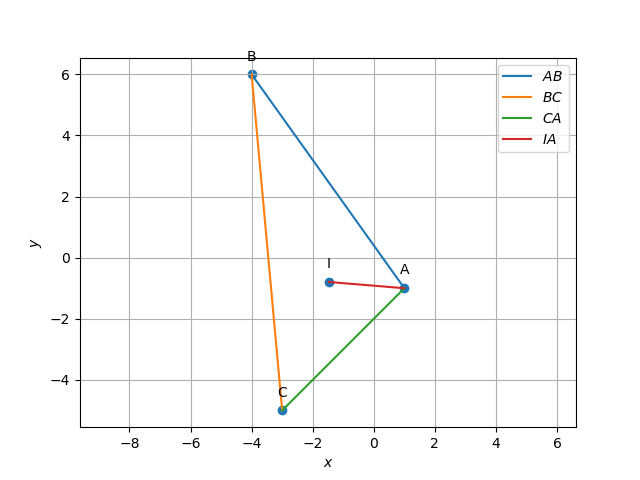
\includegraphics[scale=0.2]{main.png}}\vspace{2mm}\\
\centering{Figure}\vspace{2mm}\\
\centering \large\textsc{3  C}\footnotesize\textsc{ONSTRUCTION}\vspace{5mm}\\
\raggedright\large{The concentric circles and tangents are constructed with,} 
\begin{center}
    \label{tab:truthtable}
    \setlength{\arrayrulewidth}{0.2mm}
\setlength{\tabcolsep}{5pt}
\renewcommand{\arraystretch}{1.25}
    \begin{tabular}{|c|c|c|}
    \hline % <-- Alignments: 1st column left, 2nd middle and 3rd right, with vertical lines in between
      \large\textbf{Symbol} & \large\textbf{Co-ordinates} & \large\textbf{Description}\\
      \hline
       \large r1& 4& \large{radius}\\
       \large r2& 6& \large{radius}\\
       \large d & 6 & OP\\
	\large m1 & $\ \begin{pmatrix} 1\\\frac{2}{\sqrt{5}} \end{pmatrix}$ & \large direction vector of PQ1\\
	\large m2 & $\ \begin{pmatrix} 1\\\frac{-2}{\sqrt{5}} \end{pmatrix}$ & \large direction vector of PQ2\\
        \large$ \mu_1$ & $\frac{10}{3}$ & \large{root}\\
	\large $\mu_2$ & $\frac{10}{3}$ & \large{root}\\
        \large P & $\ \begin{pmatrix} 0\\0 \end{pmatrix}$ & \large point vector P\\
	\large O & $\ \begin{pmatrix} d\\0 \end{pmatrix}$ & \large point vector O\\
	\large \textbf{Q1} & $\mu_1\vec{m1}$ & point of contact 1\\
	\large \textbf{Q2} & $\mu_2\vec{m2}$ & point of contact 2\\
      \hline
   \end{tabular}
 \end{center}\vspace{5mm}
\raggedright\large{The figure above is generated using python code provided in the below source code link.}\vspace{2mm}\\
\begin{mdframed}
\raggedright\large{https://github.com/madind5668 \\ /FWC/blob/main/matrices/circles \\ /codes/main.py}
\end{mdframed}
\end{multicols}
\end{document}
\fi

